\documentclass{article}
\usepackage[utf8]{inputenc}
\usepackage[margin=1in]{geometry}
\usepackage{mathptmx}
\usepackage{mathtools}
\usepackage{subcaption}
\setlength{\parindent}{0em}
\setlength{\parskip}{0.5em}


\title{Assignment 2 - CTA200H}
\author{Mukesh Taank (mtaank)}
\date{May 8, 2020}

\usepackage{natbib}
\usepackage{graphicx}

\begin{document}

\maketitle

\section*{Question 1}

This question deals with looking at plotting points on the complex plane. 
We are given our initial starting position $z_0$ to be 0.
Then we are told to iterate according to the equation $z_{i + 1} = z_i^2 + c$.
We are also told to focus the area of the plane: $-2 < x < 2$ and $-2 < y < 2$.
I used about 1 million points in this region and made sure to check if they remained in the region, or if they diverged to infinity.
The following plot shows the iterations of the chosen points using the initial start at zero.

\begin{figure}[!htb]
    \centering
    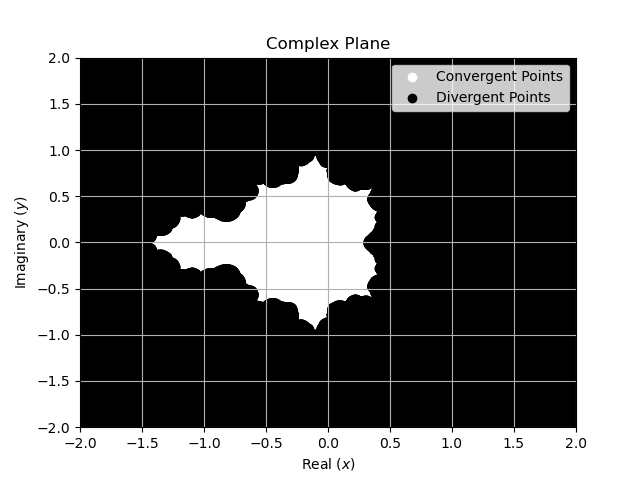
\includegraphics[scale=0.9]{Q1_updated plot.png}
    \caption{Plot of the complex plane. Points are coloured based on if the iteration diverged to infinity, or was contained within $|z|$.}
    \label{fig:Q1_plot1.png}
\end{figure}

One thing I notice is that the closer the points are to the origin, the less likely they will be to diverge. This could be due to the modulus of the numbers is relatively low, so when they are iterated, they will not go up very much. Some other points, like closer to the bounds, will have higher moduli, so when they are iterated, they will grow much more rapidly and reach large numbers.
\newpage

The next part of this question was to look at the divergent points and see the iteration number at which they broke out of the region. The following plot shows the colour bar of the iterations.

\begin{figure}[!htb]
    \centering
    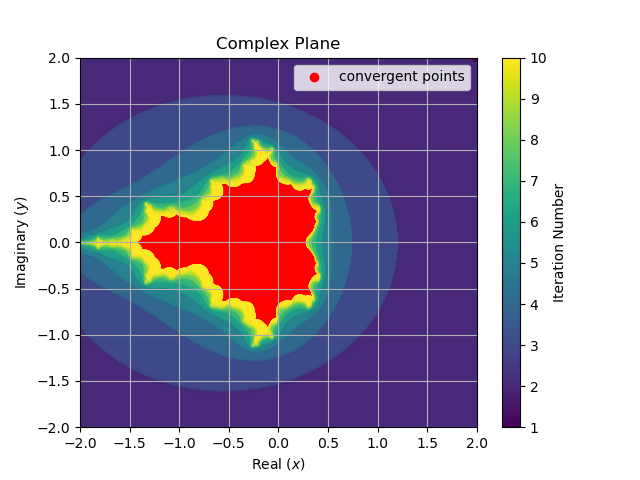
\includegraphics[scale=0.9]{Q1_updated1 plot.png}
    \caption{Plot of the complex plane, showing the iterations of the equation above using a colour scale to represent the current iteration.}
    \label{fig:Q1_plot2.png}
\end{figure}

The convergent points are represented by red. After an infinite number of iterations, they still would not diverge, so I chose to represent them by a different colour than on the colour bar. For the divergent points, the darker points represent the numbers C that cause the iteration to diverge beyond the region very quickly (within 2-3 iterations). The lighter points closer to yellow represent the numbers C that cause the iteration to diverge beyond the region slower (within 7-10 iterations).
From this, we see that the divergent points closer to the convergent points actually diverge a lot slower than the points further out. This makes sense based on looking at the relative moduli of the numbers. Points with a higher modulus will increase and diverge faster than points with lower moduli.
\newpage

\section*{Question 2}

This question deals with looking at the SIR model, which is a simple mathematical model of disease spread in a population. 
We are given a set of ordinary differential equations by which this spread is modelled by. 
Using the given initial conditions and differential equations, I was able to use an ODE integrator to solve for the $S$, $I$ and $R$ functions to get their relations with respect to time.
One thing that needed to be done first was to find realistic values for the parameters $\beta$ and $\gamma$. 

$\beta$ represents the rate of the spread of infection per contact between infected and non-infected per unit time.
$\gamma$ represents the rate at which the infected recover per unit time.

From this, I can assume reasonable values for $\beta$ and $\gamma$, which are between 0 and 1. 
If we assume beta is, for example, 0.5, then this is saying that the disease is spread through 1 meeting between the infected and non-infected every 2 days. 
If we assume gamma is, for example, 0.5, then this is saying one person will recover every 2 days.

To approach this problem, I used the built-in function in SciPy: scipy.integrate.odeint() in order to solve the set of differential equations.
When I solved the set of ODEs and finally got my solution functions, I then plotted them onto one graph using varying values for $\gamma$ and $\gamma$ to see how the curves would change with respect to these parameters.
The following figures show the plots of $S(t)$, $I(t)$ and $R(t)$ with different values of $\beta$ and $\gamma$.

\begin{figure}[!htb]
  \centering
  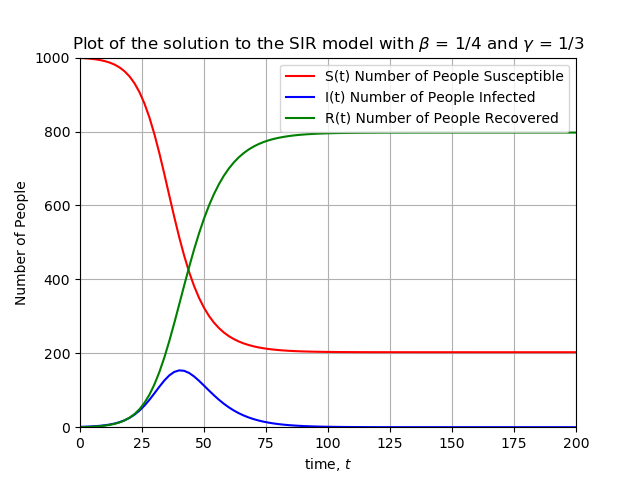
\includegraphics[width=1\linewidth]{Q2_plot1.png}
  \caption{Plot of the solution functions; $S(t)$, $I(t)$ and $R(t)$ \\ over time, with $\beta$ = 1/6 and $\gamma$ = 1/3.}
  \label{fig:Q2_plot1.png}
\end{figure}

Looking at Figure 3, we have a $\beta$ value of 1/6 and a $\gamma$ value of 1/3. 
So in this case, $\beta$ $<$ $\gamma$.
From this relation, we see that the peak of the number of people infected is about 170, and happens around day number 43.
The number of people susceptible and number of people recovered actually equal at  about day 42.
In this case, the peak number of infected people is relatively low.
\bigskip

\begin{figure}[!htb]
  \centering
  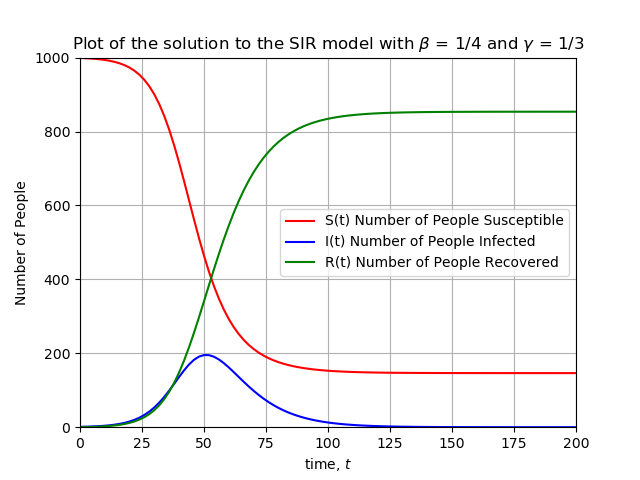
\includegraphics[width=1\linewidth]{Q2_plot2.png}
  \caption{Plot of the solution functions; $S(t)$, $I(t)$ and $R(t)$ \\ over time, with $\beta$ = 1/9 and $\gamma$ = 1/4.}
  \label{fig:Q2_plot2.png}
\end{figure}

In Figure 4, we have a $\beta$ value of 1/9 and a $\gamma$ value of 1/4. 
So in this case, $\beta$ $<$ $\gamma$.
From this relation, we see that the peak of the number of people infected is about 200, and happens around day number 50.
The number of people susceptible and number of people recovered actually equal at  about day 42.
This plot is very similar to figure 4, as the general shape of the curves is consistent.
In this case, the peak number of people infected is relatively low.
\newpage

\begin{figure}[!htb]
  \centering
  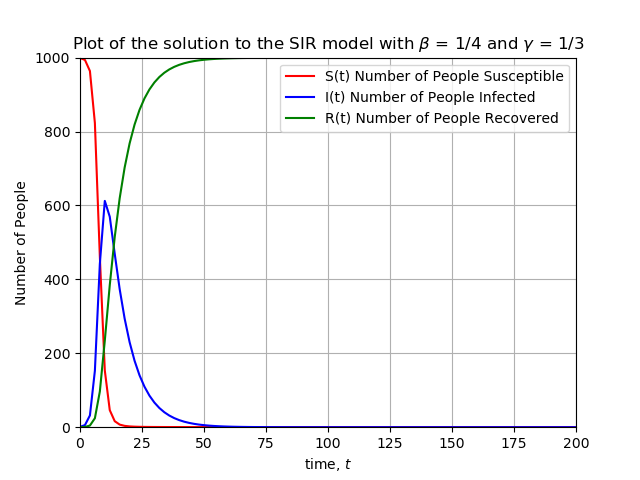
\includegraphics[width=1\linewidth]{Q2_plot3.png}
  \caption{Plot of the solution functions; $S(t)$, $I(t)$ and $R(t)$ \\ over time, with $\beta$ = 1/8 and $\gamma$ = 1.}
  \label{fig:Q2_plot3.png}
\end{figure}

In Figure 5 below, we have a $\beta$ value of 1/8 and a $\gamma$ value of 1. 
So in this case, $\beta$ $<<$ $\gamma$.
From this relation, we see that the peak of the number of people infected is about 600, and happens around day number 12.
The number of people that are susceptible to the virus decreases very fast, starts at 1000 and reaches zero in about 18 days.
This also means that the number of people that were infected did make a recovery since the recovery curve reaches the maximum of 1000.
So with this combination of $\beta$ and $\gamma$, we see a relatively high peak that occurs very fast.
Since the peak of the number of people infected happened very early, the number of people infected dropped off quickly and eventually reached zero after about 60 days.
Also, everyone is healthy from the virus/disease after the same 60 days and no one is susceptible any more.
This plot is very similar to figure 4, as the general shape of the curves is consistent.
In this case, the peak number of people infected is relatively high.
\newpage

\begin{figure}[!htb]
  \centering
  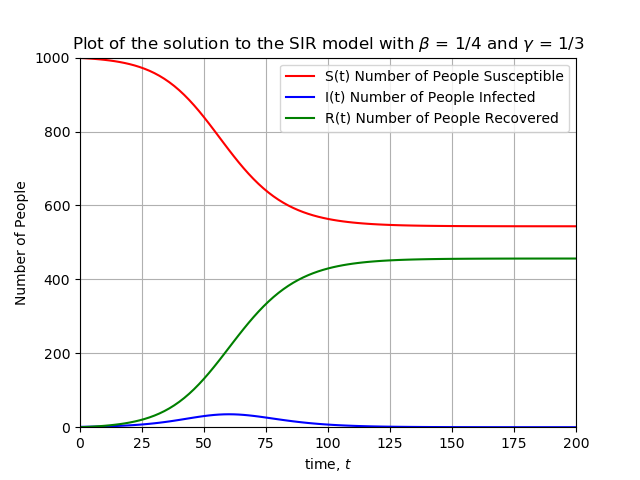
\includegraphics[width=1\linewidth]{Q2_plot4.png}
  \caption{Plot of the solution functions; $S(t)$, $I(t)$ and $R(t)$ \\ over time, with $\beta$ = 1/4 and $\gamma$ = 1/3.}
  \label{fig:Q2_plot4.png}
\end{figure}

In Figure 6, we have a $\beta$ value of 1/4 and a $\gamma$ value of 1/3. 
So in this case, $\beta$ $\approx$ $\gamma$.
From this relation, we see that the peak of the number of people infected is only about 30 people, and happens around day number 60.
So with this combination of $\beta$ and $\gamma$, we see a very low peak, indicating that the virus is not spreading very fast at all.
After around 110 days, there are no longer any people infected.One thing that is different in this graph compared to the others is that the number of people susceptible and the number of people the recover, are never equal. Since not many people get infected in the first place, the number of susceptible people goes down relatively fast and the opposite for the number of people recovered, it goes up relatively quickly.
This plot is very similar to figure 4, as the general shape of the curves is consistent.
In this case, the peak number of people infected is relatively high.

From analyzing the different variations of $\beta$ and $\gamma$, we can see how likely a virus/disease is to spread among a given population given the amount of times people are in contact with each other (which comes from the two parameters).


\end{document}